\section{Average Word Length (AWL) analysis}
\subsection{First results}
The Average Word Length (hereinafter called AWL) of a text is defined as the number of characters in a text divided by the number of words.
After calculating and plotting the AWL of all collections in the Pali canon, the following chart ensued:\\

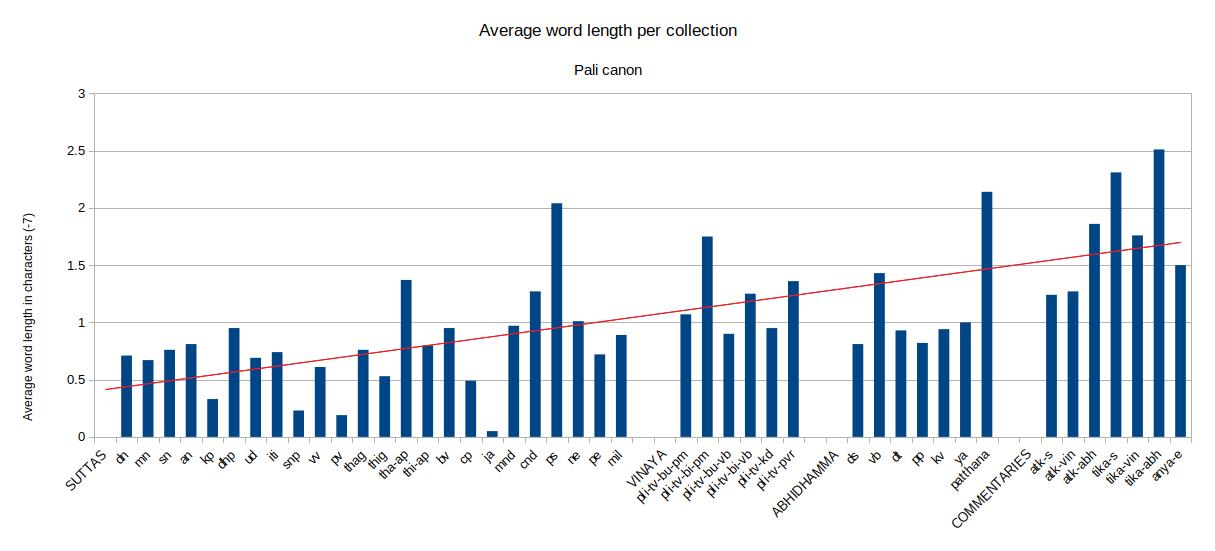
\includegraphics[width=\linewidth]{chart1.jpg}
\captionof{figure}{The AWL in characters above 7 per collection in the Pali canon.}
\label{chart1}

\medskip
Some interesting things can be seen from this chart. First of all, it is clear that most collections that are generally accepted as "Early Buddhist Texts (EBTs)"--the first four Nikāyas and the first 9 collections in the Khuddaka Nikāya with the exception of the Vimānavatthu and Petavatthu\footnote{{\em The Authenticity of the Early Buddhist Texts} by Bhikkhu Sujato and Bhikkhu Brahmali}--have a lower AWL while the later commentarial texts have a much higher AWL.

The Vinaya and Abhidhamma texts as well as the later Sutta texts seem to be in between with roughly the same range of AWL, indicating that these texts might have developed over a period of time thereafter. There are also some collections that do not match this broad pattern and I will discuss these below.

Especially the relative high value of the Dhammapada (dhp) is surprising because the Dhammapada is generally seen as one of the earliest Buddhist texts. Then there are other discrepancies like the Jātaka (ja) and the Bhikkhunī Pātimokkha (pli-tv-bi-pm). So I will explore these in more detail below.

\subsection{The influence of headings}
Analysing the Dhammapada (dhp) (\url{https://suttacentral.net/dhp/pli/ms}), I noticed that especially the headings have a much larger word-length than the verses. 

If we keep in mind that all early texts were only transmitted orally and organized and written down at a much later date, it is likely that headings were inserted into the texts later, when these texts were scripturalized.

So calculating the same chart with the headers removed gives the following chart:\\

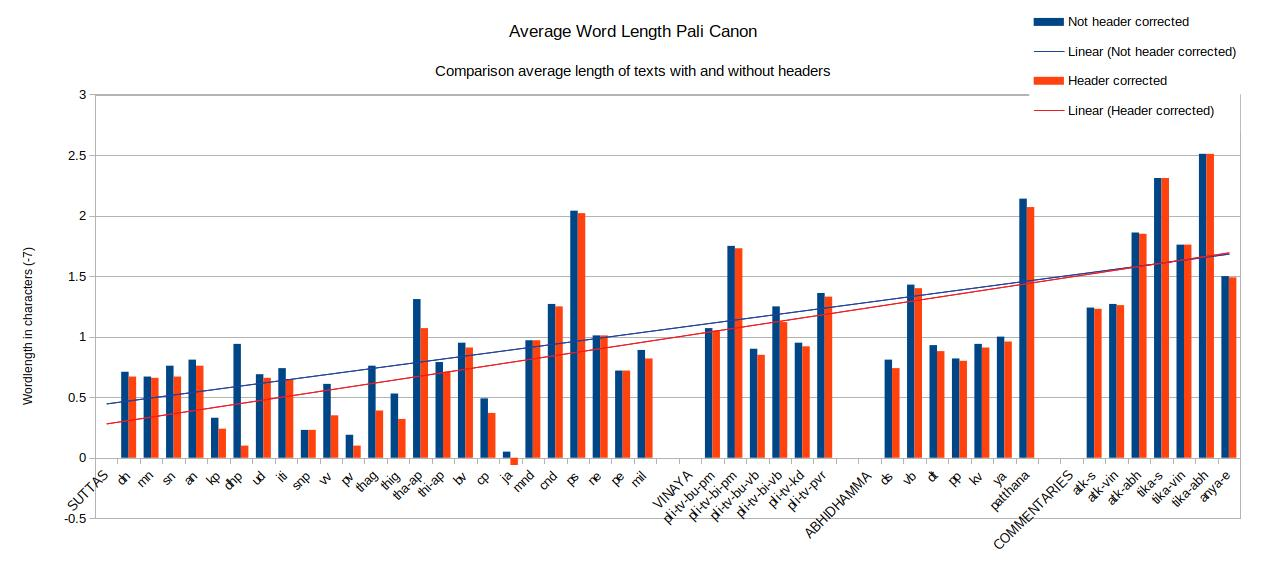
\includegraphics[width=\linewidth]{chart2.jpg}
\captionof{figure}{The AWL in characters above 7 per collection in the Pali canon comparing calculations with and without headers.}
\label{chart2}

\medskip
Removing headers from the calculation and just analysing the prose or verse text gives a very different picture for expecially the Dhammapada, which has now jumped from a relatively high value to a much lower value which is much more in line with our accepted understanding of the Dhammapada as a very early text.

Another interesting thing we see in this chart is that removing the headers has a much more dramatic effect on the Early Buddhist texts and the commentarial texts are hardly affected. So it seems safe to assume that headers are indeed inserted into the texts later.

\subsection{Verse, prose and mātikā}
When we look at the charts, we have to be aware that there are different types of texts, which due to their nature have higher or lower values of the AWL overall. 

Collections with predominantly verses have a much lower AWL than collections with prose, also those that are regarded as late. It might be that verse, by its very nature, needs shorter words. But this is not always the case as we will see in the analysis of the Jātaka. Due to the history of oral tradition, it was much easier to remember and recite verses than prose and we do indeed see that verse summaries of prose teachings were one method to ensure oral transmission.

Mātikā are yet a very different type of text that is mainly used in the Abhidhamma. These are lists of contents or matrix which make use of shorter words then regular text. The Dhammasaṅgaṇī clearly illustrates this and therefore has a lower AWL.

In the following chart we can see this difference a bit more clearly, using a different scale to the previous charts. Here the y-axis shows the AWL in characters above 7.76 so the EBT collections all get a negative value.\\

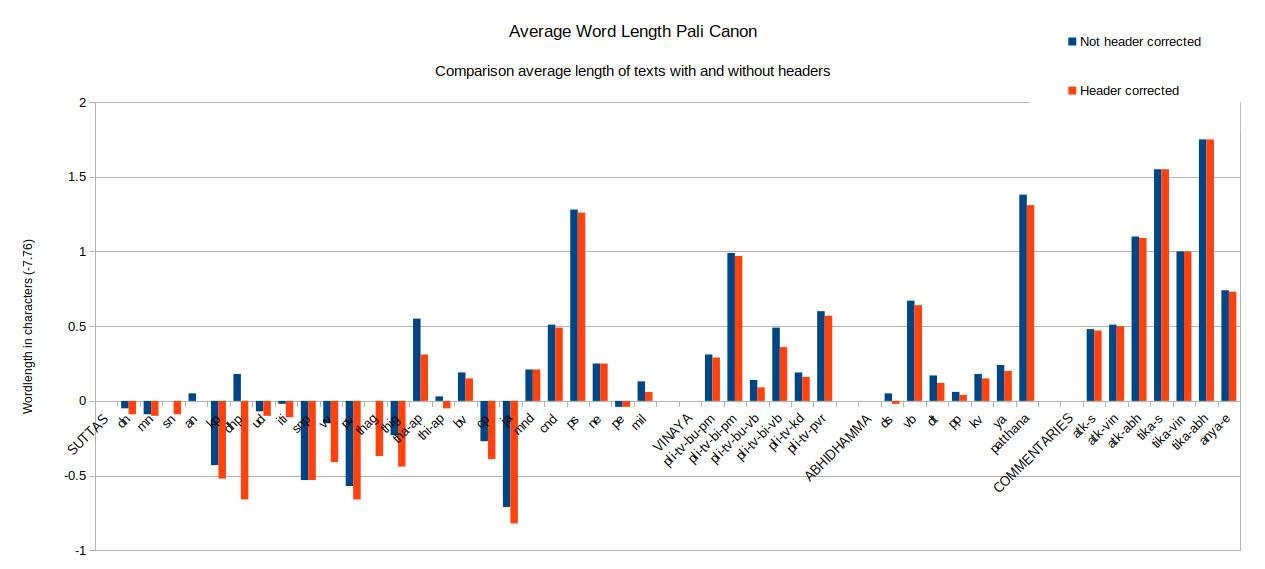
\includegraphics[width=\linewidth]{chart3.jpg}
\captionof{figure}{The AWL in characters above 7.76 per collection in the Pali canon comparing calculations with and without headers.}
\label{chart3}

\medskip
The value of 7.76 is chosen because this is the highest value for the AWL of all the EBTs, corrected for headers. This is, maybe not surprisingly, the value of the Aṅguttara Nikāya. This value is consistent with our understanding that from all the EBTs the Aṅguttara Nikāya has been influenced most by later insertions.

\subsection{Collections with a very high or low value}
There are several collections that show a surprising high or low value of AWL in the chart and I will analyse each of these below.

\subsubsection{Dhammapada (dhp)}
The Pali version of this famous text, consisting of 423 verses organized into memorable themes. It is the most widely read of the early texts, and has been translated many times into many languages. Versions of this text are found in Chinese, Tibetan, and several Indic languages, attesting to its timeless, universal appeal. The Dhammapada is a very early text; some of the verses have parallels with Vedic texts (i.e. Mahābhārata, Garuḍapurāṇa and Manusmṛti) and Jaina texts (i.e. Uttarādhyayanasūtraṁ, Isibhāsiyāiṁ).

The following table shows the AWL of the DHP verses that have parallels with Vedic and Jaina texts in both the Mahāsaṅgīti edition and the Comparative Edition of the Dhammapada by Ānandajoti Bhikkhu\footnote{The Dhammapada, A New Edition edited by Ānandajoti Bhikkhu. URL: \url{https://www.ancient-buddhist-texts.net/Buddhist-Texts/K2-Dhammapada-New/index.htm} The text of the Dhammapada in this new edition has been established through a comparison of the Sinhalese, Burmese, Thai, and European editions.}.\\

\small
\begin{tabular}{ l c c l }
\textbf{Verse} & \textbf{AWL Mahāsaṅgīti} & \textbf{AWL Ānandajoti} & \textbf{Parallels} \\
dhp47 & 7.27 & 6.67 & Mahābhārata \\
dhp70 & 6.50 & 6.50 & Uttarādhyayanasūtraṁ, Isibhāsiyāiṁ \\
dhp103 & 6.64 & 5.54 & Uttarādhyayanasūtraṁ \\
dhp128 & 6.69 & 7.20 & Garuḍapurāṇa \\
dhp131 & 6.25 & 5.77 & Mahābhārata, Manusmṛti \\
dhp200 & 6.50 & 6.50 & Mahābhārata, Uttarādhyayanasūtra \\
dhp223 & 7.40 & 6.82 & Mahābhārata \\
dhp260 & 5.14 & 5.38 & Manusmṛti \\
dhp285 & 8.90 & 6.80 & Uttarādhyayanasūtraṁ \\
dhp287 & 7.90 & 7.18 & Mahābhārata
\end{tabular}

\normalsize
\medskip
This table shows that in the Mahāsaṅgīti version as used for this analysis, most DHP verses with parallels in Vedic and Jaina texts have an AWL lower than the average of 7.1. This can be an indication but we have to be very careful drawing any definate conclusions from this; this dataset is too small to be statistically significant but it is an example. The Vedic and Jaina texts were not closed texts at the time of the Buddha either and they have seen changes and compilations at a later date so it is hard to say which text borrowed from which. As the comparison of the AWL with the Comparative Edition shows, in various editions the verses are written differently, which gives a different value for the AWL.

We cannot make any assertions about the lateness or earlyness of individual suttas or verses based on the AWL, but we can use it as an indication together with other indications or to show a general trend.

\subsubsection{Jātaka (ja)}
A collection of 547 sets of verses telling stories of the Buddha’s past lives. The canonical Pali collection consists of verses arranged in numbered sets in the Aṅguttara fashion. The shorter sets illustrate a high point of a story, while the longer sets tell a complete story. These verses would have been passed down from the beginning with prose narrative to flesh out the story, which in the Pali is now found in the commentary. It is in the commentary that we find the explicit connection between the stories of the past and the present day, identifying the hero of the tale with the bodhisattva and the major protagonists with the Buddha’s contemporaries. This collection is the main source of Jātakas, but there are many similar stories found elsewhere in the Pali canon (a few in the four nikāyas, others in the Cariyapiṭaka) and throughout the Chinese, Tibetan, and Sanskrit texts. Most of the Jātakas began life as folk tales or myths, drops from the vast ocean of story in oral culture. Several Jātakas record versions of famous Hindu myths, while others share a common basis with European folk tales. The verse forms in the Jātakas are mostly of the earlier kinds, and the social and political reflect historical realities in the centuries before the Buddha, where, for example, Varanasi was an independent kingdom. The Jātakas are the oldest, largest, and best-preserved collection of ancient stories found anywhere in the world. 

One of the most striking anomalies in the AWL is the Jātaka collection. In fact, it is the collection with by far the lowest AWL. This is maybe not so surprising given the history of these tales from mainly pre-Buddhist sources and therefore an earlier use of the Pali language, resulting in a shorter overall word-length. However, this does not explain the very low AWL value of some of the other late verse-collections.

The below figure shows the distribution of the Jātakas.\\

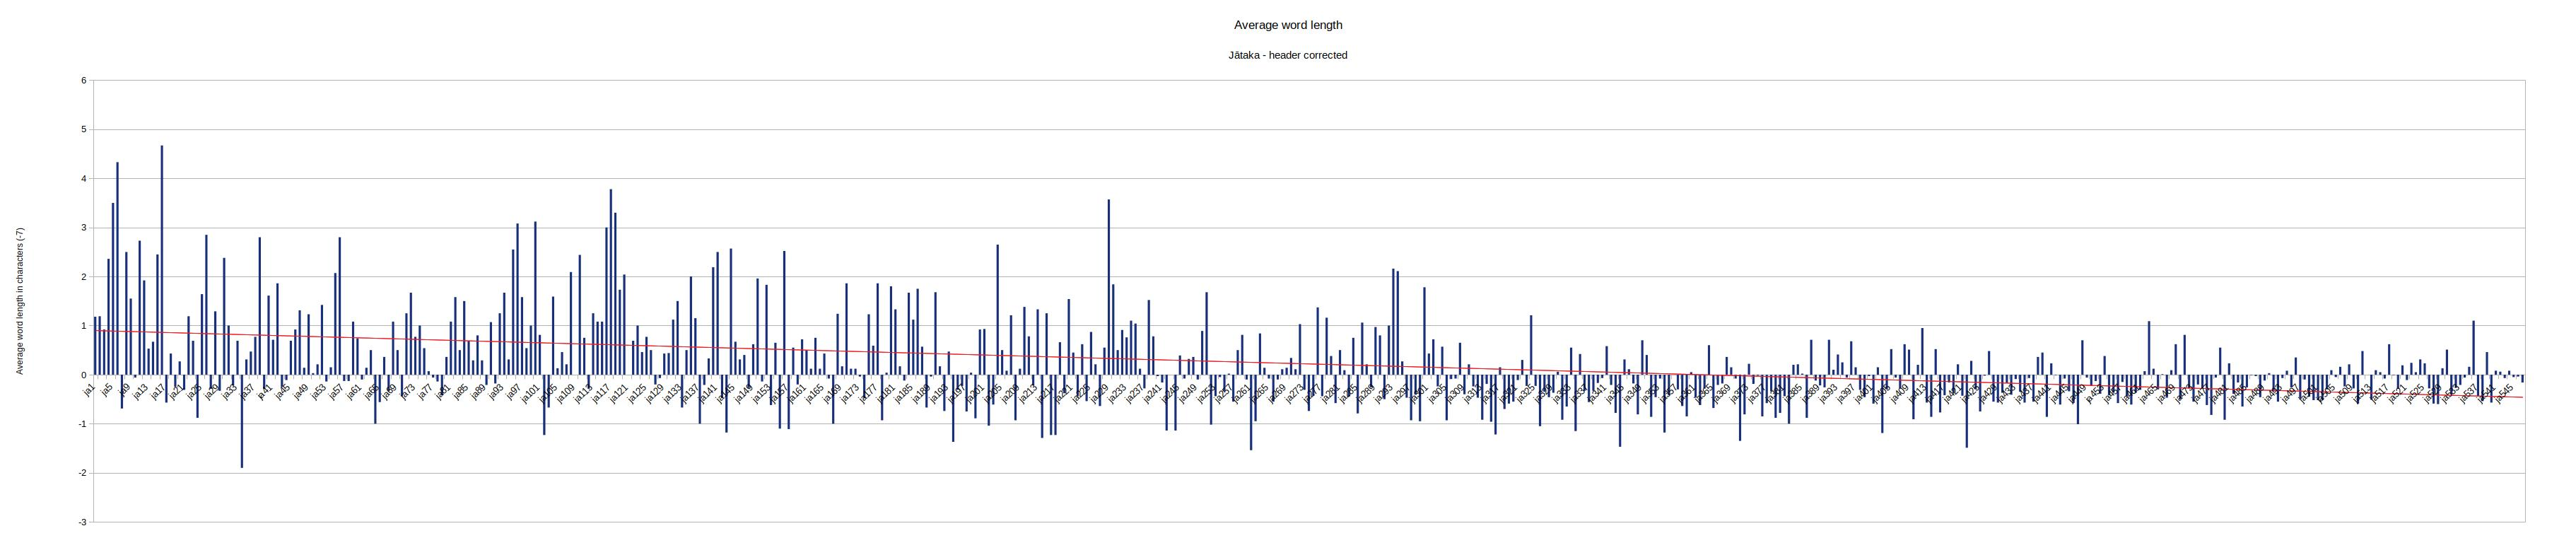
\includegraphics[width=\linewidth]{jataka.jpg}
\captionof{figure}{The AWL in characters above 7 per collection in the Pali canon comparing calculations with and without headers. The red line shows the linear trendline (regression through equation y=a*x+b)}
\label{jataka}

\medskip
This figure shows an interesting trend: the shorter Jātakas with a lower number seem to have a much higher word-length on average than the ones further in the collection. 

The next figure shows the number of parallels listed on SuttaCentral for the texts in this collection on a logarithmic scale. \\

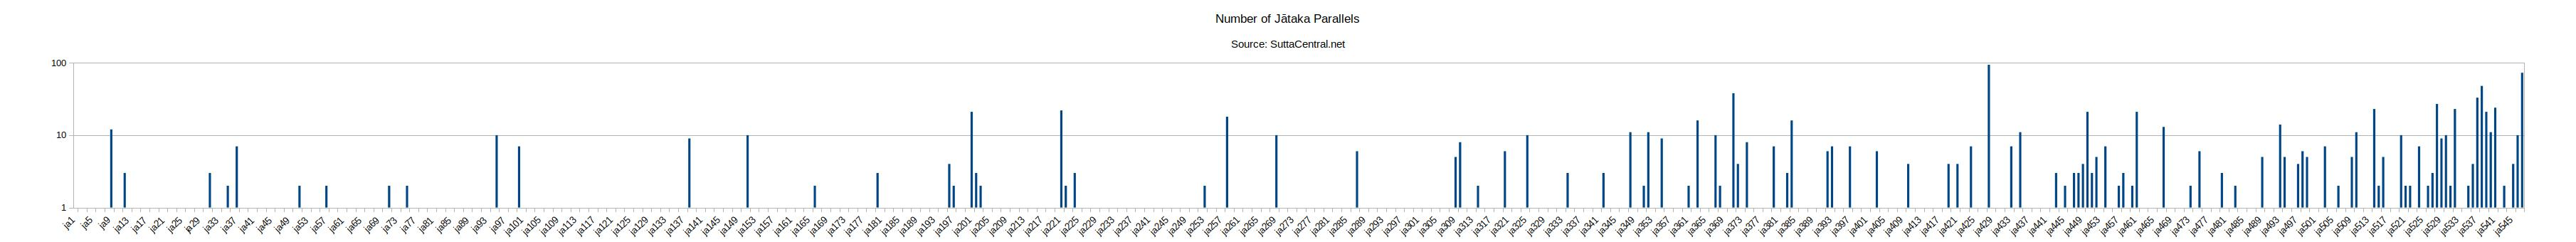
\includegraphics[width=\linewidth]{jatakapars.jpg}
\captionof{figure}{The number of parallels as listed on SuttaCentral on a logarithmic scale}
\label{jatakapars}

\medskip
Although there are not very many known parallels for many of these texts, it is clear from this that the most parallels appear in the higher end of the Jātaka collection, where the complete story is told.

From both of these charts it would seem that the Jātaka with a higher number are likely to be earlier than the first part of the collection. Of course we cannot make any assumptions about the lateness or earlyness of individual suttas based on this method, especially if many of these only contain just one verse, but it is an indication of a general trend.

\subsubsection{Vimānavatthu (vv) and Petavatthu (pv)}
The “Stories of Celestial Mansions” contains 85 stories in verse that illustrate the heavenly rewards of virtuous deeds, especially making offerings to the Buddha or the Saṅgha. The Stories of Hungry Ghosts” contains 51 stories in verse that illustrate rebirth as a hungry ghost as a result of bad deeds.

The most striking about the Vimānavatthu and Petavatthu is that they seem to fit seemlessly into the graph as part of the EBTs according to their AWL. Yet they are late devotional texts with no direct counterparts in other collections.

In how far the low AWL value has to be sought in the fact that these are verse collections I cannot tell. Another possibility is that in order to be consistent, the authors of these texts have gone through considerable length to use a language that was more consistent with the early texts; it might be an attempt to make the texts look genuine. More research will need to be done to find an answer to this question.

\subsubsection{Therāpadāna (tha-ap) and Therīapadāna (thi-ap)}
The “Legends of the Senior Monks” and the “Legends of the Senior Nuns” contain 563 and 40 stories resp. in verse telling the past life deeds of various senior monks/nuns. These are a much later counterpart to the Theragāthā and Therīgāthā, referring to many of the same monks/nuns. But whereas the Theragāthā/Therīgāthā verses relate the monks’ and nuns’ practice of meditation and mindfulness in this life, the Legends typically relate how they became awakened in this life by making an offering a Buddha in the distant past, and making a dedication to be reborn so as to become awakened in the future. Both these are late texts, and lack counterparts in the northern canons.

In analysing this text I can find no reason for the relatively low value of the AWL for the Therīapadāna in comparison to the Therāpadāna. It seems however that the last part of the Therāpadana is slightly lower in AWL and more consistent with the low value of the Therīapadāna.

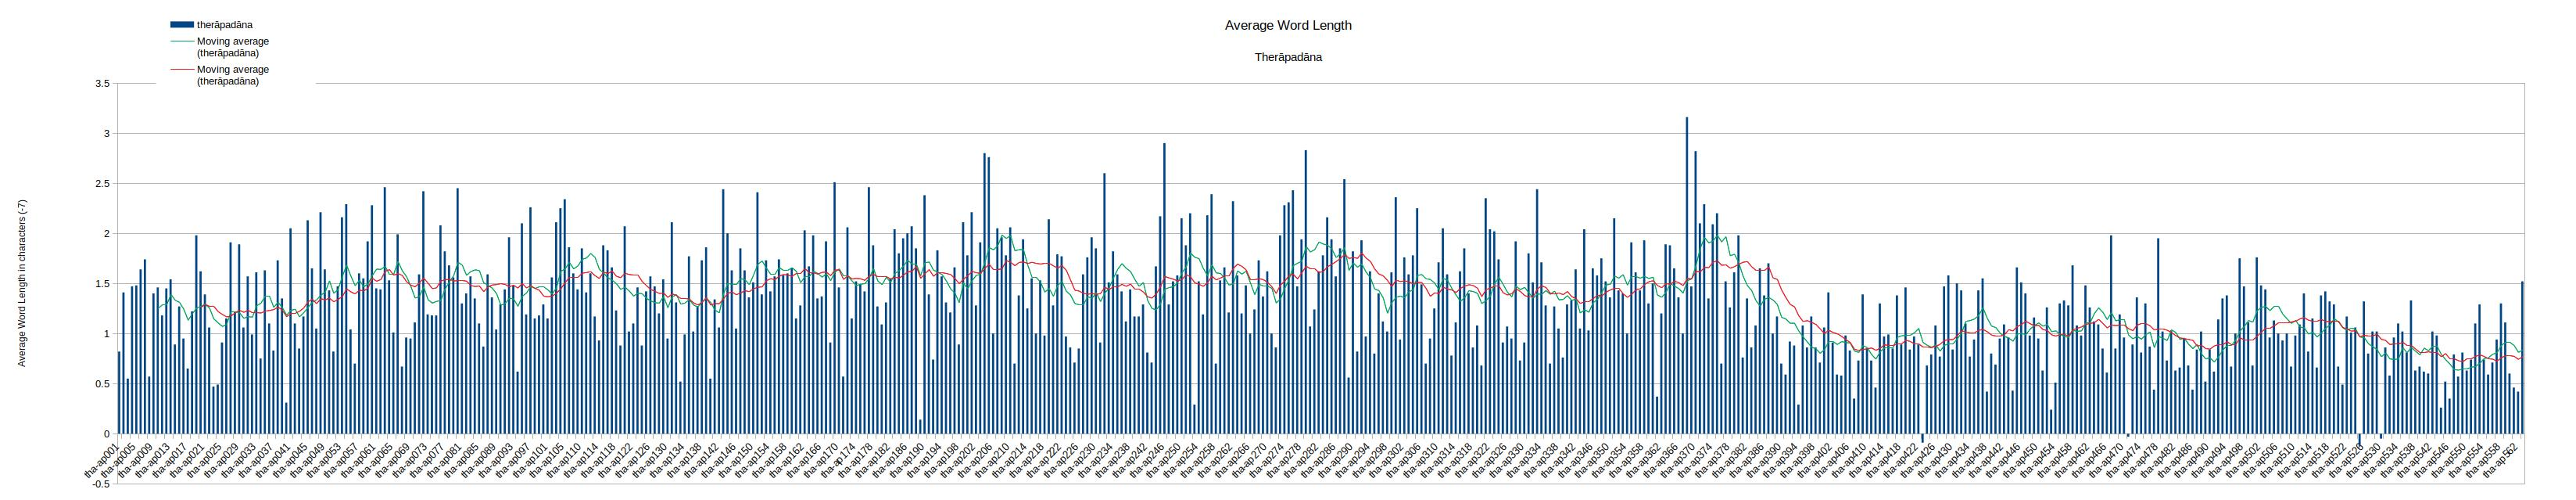
\includegraphics[width=\linewidth]{thaap.jpg}
\captionof{figure}{Therāpadāna AWL values with moving average lines (green = period 10, red = period 20)}
\label{thaap}

\medskip
Around the Pilindavaccha Vagga the AWL value makes a drop as is also clear from the moving average lines. From this point onwards, the AWL values of the Therāpadāna are much more consistent with the Therīapadāna as the following chart shows. This might indicate that these parts are slightly earlier and that the first parts of the Therāpadāna (with shorter texts) was added later.\\

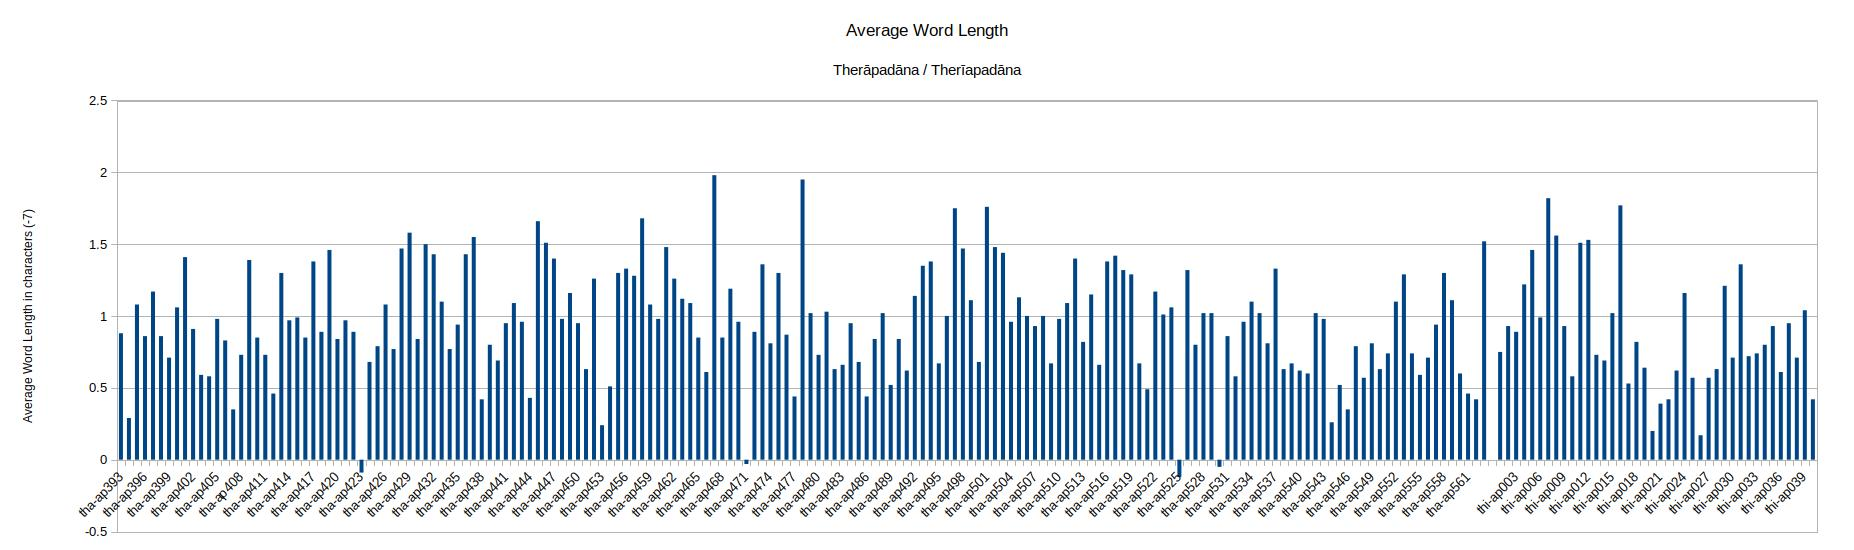
\includegraphics[width=\linewidth]{thaiap.jpg}
\captionof{figure}{Therāpadāna AWL from Pilindavaccha Vagga onwards in comparison to the Therīapadāna}
\label{thaiap}

\subsubsection{Cariyāpiṭaka (cp) and Buddhavaṃsa (bv)}
Another interesting collection as is seen in figure \ref{chart3} is the Cariyāpiṭaka. 

The “Basket of Conduct” represents an early systematization of the concept of the Bodhisattva and his path towards awakening. A selection of 34 past lives are told, each one illustrating a specific virtue developed by the Bodhisattva. It is a late text, without direct counterparts in the northern collections. Like the Buddhavaṃsa, a late devotional text in verse detailing the lives of 24 past Buddhas and the prediction of the awakening of the historical Buddha Gotama, it is part of an extensive pan-sectarian devotional literature composed in the second and first centuries BCE, presaging the birth of the Mahāyāna.

The Cariyāpiṭaka mainly comprises of retellings of the Jātaka stories. Analysing this in a chart we get the following:\\

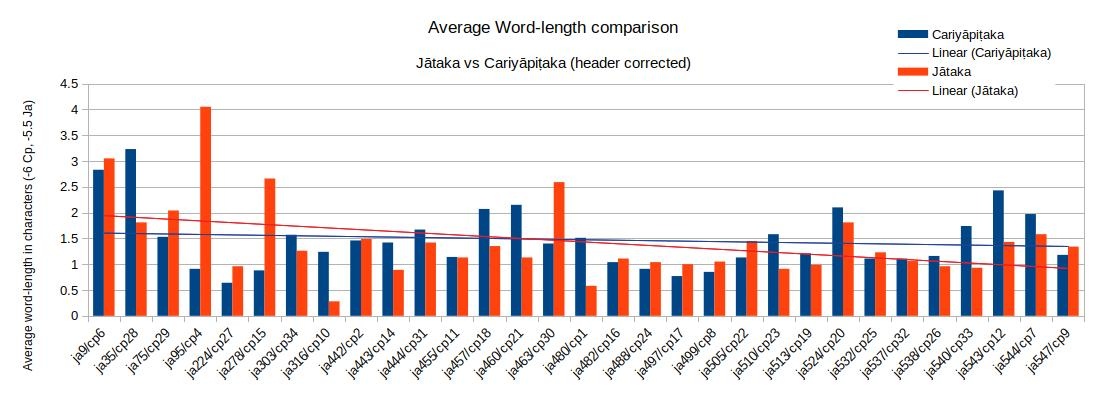
\includegraphics[width=\linewidth]{jacp.jpg}
\captionof{figure}{Comparison of Jātaka with Cariyāpiṭaka (Note that for the purpose of this comparison the value of length for Cariyāpiṭaka is .5 characters higher than for Jātaka)}
\label{jacp}

\medskip
There seems to be a rough, but not entirely convincing, similar trend between the two collections. More notably we see that most of the Cariyāpiṭaka are retellings of the Jātaka with higher numbers. 

Although at present I do not have a convincing explanation as to why the Cariyāpiṭaka, unlike the Buddhavaṃsa, would have such a very low AWL, given it's age but I suspect it's correlation to the Jātaka might have something to do with it.\\

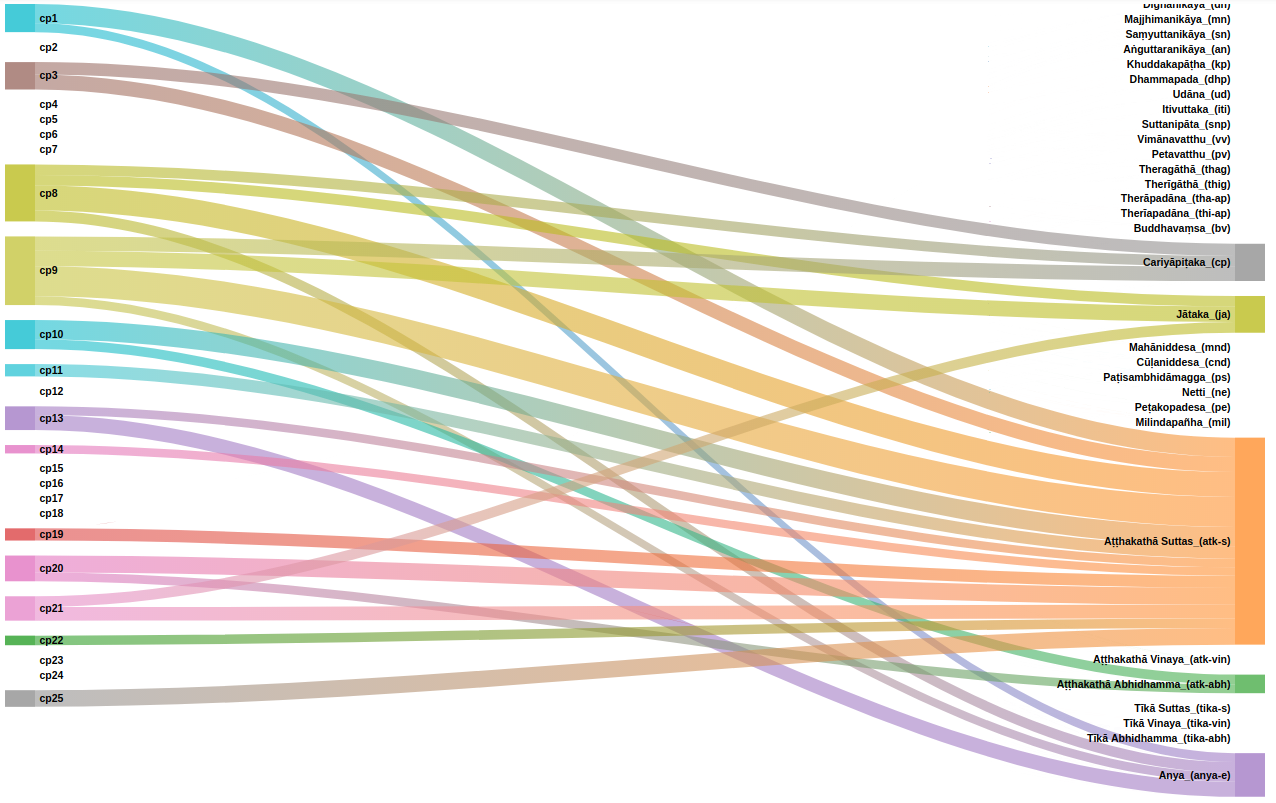
\includegraphics[width=\linewidth]{cp.png}
\captionof{figure}{Cariyāpiṭaka sankey chart showing connections with other collections}
\label{cp}

\medskip
Both collections are vastly different from the other collections. The sankey charts \ref{cp} and \ref{bv} show there are no matches found between them and other collections, indicating a completely different use of language. The same pattern we also see for the Therāpadāna, Theriapadāna and to a lesser extend for the Vimānavatthu and Petavatthu.\\

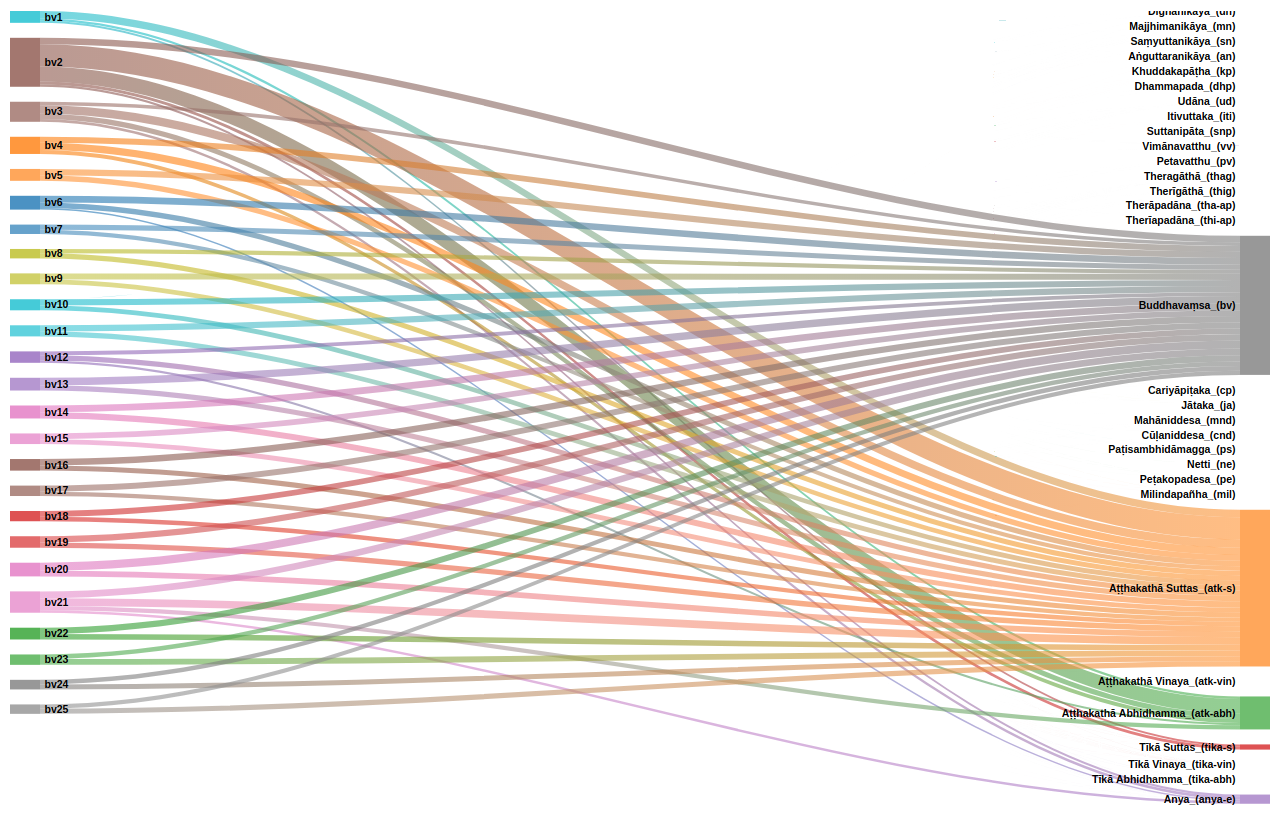
\includegraphics[width=\linewidth]{bv.png}
\captionof{figure}{Buddhavaṃsa sankey chart showing connections with other collections}
\label{bv}

\medskip
Note that the Buddhavaṃsa seems to be highly repetitive across the various texts in this collection.

The only matches found are with the commentaries and most notably with the Aṭṭhakathā Suttas. The major commentaries were based on earlier ones, now lost, in Prakrit and Sinhala, which were written down at the same time as the Canon, in the last century BCE. Would it be possible therefore that the Cariyāpiṭaka and Buddhavaṃsa were part of the lost early commentaries?

\subsubsection{Paṭisambhidāmagga (ps)}
The Paṭisambhidāmagga or “Path of Analytical Discernment” is an advanced critical treatise in thirty chapters on Buddhist practice, which the Pali commentaries attribute to the Buddha’s disciple Sāriputta. Departing from the popular or folksy style of most Khuddaka texts, it is more reminiscent of the Abhidhamma, and indeed, while not included in the Abhidhammapiṭaka, it deserves to be considered part of the Theravādin Abhidhamma system. However, it does not make use of the main Abhidhamma mātikās. This text introduces a number of terms and ideas of great importance in later Buddhist philosophy. It does not have any counterparts in the northern canons, but articulates a dictinctly Theravādin perspective on the path.

The history of this text shows indeed in it's very high AWL value. The AWL value is however higher than most Abhidhamma collections so it might be possible that this text has developed in a very late stage.

\subsubsection{Peṭakopadesa (pe)}
The Peṭakopadesa or “Illustration of the Baskets” is a systematic treatise intended to provide a guide for reading and interpreting the texts of the nikāyas. It is similar to the Netti, and the exact relationship between these two texts is not clear. The text provides an array of methods for reading texts, illustrating them with quotations, and taking the four noble truths as the overall framework. The Pali text of the Peṭakopadesa is quite corrupt, which is unusual in the Pali canon. A colophon in the text attributes it to the Buddha's disciple Kaccāna. It is, however, a late text, lacking counterparts in the northern collections. It is not universally accepted as canonical; SuttaCentral’s Pali texts, however, stem from the Mahāsaṅgīti edition, which as a Burmese text does include it.

As this text is not universally accepted as canonical, I will disregard the low value of the AWL as an anomaly.

\subsubsection{Bhikkhunī Pātimokkha (pli-tv-bi-pm)}
The bhikkhunī-pātimokkha, “the monastic code for nuns,” contains the core rules of the monastic life in the form of a long list without any explanatory material. There are 311 such rules for the nuns, grouped according to the type of offense incurred for breaking the rule, with the exception of the last group, the adhikaraṇasamathadhamma (“the principles for resolving legal issues”), which are principles to be applied rather than rules in the strict sense.

The AWL of the Bhikkhunī Pātimokkha seems very high in comparison to the other collections of the Vinaya. This is not surprising if we remember that the Bhikkhunī Pātimokkha had been lost and was actually reconstructed from a commentarial text. No doubt due to it's history, the text would also have acquired some of it's later use of the Pali language, most notably with compounds and therefore longer words. This does not say anything about the actual age of the original Bhikkhunī Pātimokkha, only of the current version we have.

\subsubsection{Parivāra (pli-tv-pvr)}
The Parivāra, “the Compendium,” is a technical analysis of the content of the Suttavibhaṅga and the Khandhakas. It summarizes and distils the essence of the Vinaya, leaving out all narratives and stories. One example of its approach is an Aṅguttara-nikāya style chapter, where aspects of the Vinaya are summarized in bare numerical lists. Towards the end of the Parivāra we find a chapter entertainingly named the Sedamocakagāthā, “the Sweat-inducing verses,” which consists of a series of difficult riddles to be solved by advanced students of the monastic law.

The Parivāra is unique to the Theravada school and it is probable that it was compiled in the sectarian period. Its manner of analysis shares certain characteristics with the Abhidhamma, such as expanding and filling in schemes of classification not given in full detail in the other Canonical texts. One example is the Parivāra’s exposition of the “sources of offenses,” āpattisamuṭṭhāna, for each individual rule, with only a general scheme found in the rest of the Vinaya. The similarity of approach with the Abhidhamma could indicate that they stem from roughly from the same period. Two references to writing also suggests a relatively late composition for this work.

The high value of the AWL is consistent with the idea that this is a later text. 

\subsubsection{Dhammasaṅgaṇī (ds)}
The Dhammasaṅgaṇī (Compendium of Phenomena) is built on the idea of a mātikā, a lists of contents or matrix. A mātikā acts as a simple instance of a template that is applied and transformed in ever more complex forms throughout the work. The Dhammasaṅgaṇī mātikās list sets of phenomena (dhammas). Most of these are doctrinal terms familiar from the suttas, although some are specialized Abhidhamma terms. The Dhammasaṅgaṇī starts with three mātikās. The first classifies dhammas into 22 sets of three (tika), and the next two use sets of two (duka), 100 pairs for Abhidhamma terms, and 42 for Sutta terms. The first of the triple sets is the momentous group: wholesome, unwholesome, and undetermined. This serves as a framework for classifying all the various phenomena. While it seems simple enough, even this detail was controversial, as some schools rejected the existence of the undetermined, or morally neutral, category.

The low AWL value seems to have more to do with the structure of this book, comprising of mātikā, then it's age. It is therefore a vastly different way of writing than verse or prose.

\subsubsection{Vibhaṅga (vb)}
The Vibhaṅga (Book of Analysis) consists of 18 chapters arranged by topic. The list of topics is closely related to the Saṁyutta Nikāya—aggregates, senses, dependent origination, etc. Most of the chapters have a threefold structure. (1) Analysis according to the suttas: this quotes a key passage from the suttas on the relvant topic and offers a modest analysis. (2) Analysis according to the Abhidhamma: applies the sets of synonyms and terms as developed in the Dhammasaṅgaṇī. (3) Catechism: tests the students knowledge with systematic questioning. A few sections, such as Vb 18 Dhammahadaya, do not fit this system. They may have originated as independent treatises.

The Vibhaṅga, unlike the Dhammasaṅgaṇī, seems to have a much greater AWL then most of the other Abhidhamma books. 

An overview of all the matches of this text with other texts reveals the connection with the suttas as well as other Abhidhamma texts, most notably the Dhammasaṅgaṇī. This does not explain the high AWL other than that it is obviously later than the Dhammasaṅgaṇī itself.\\

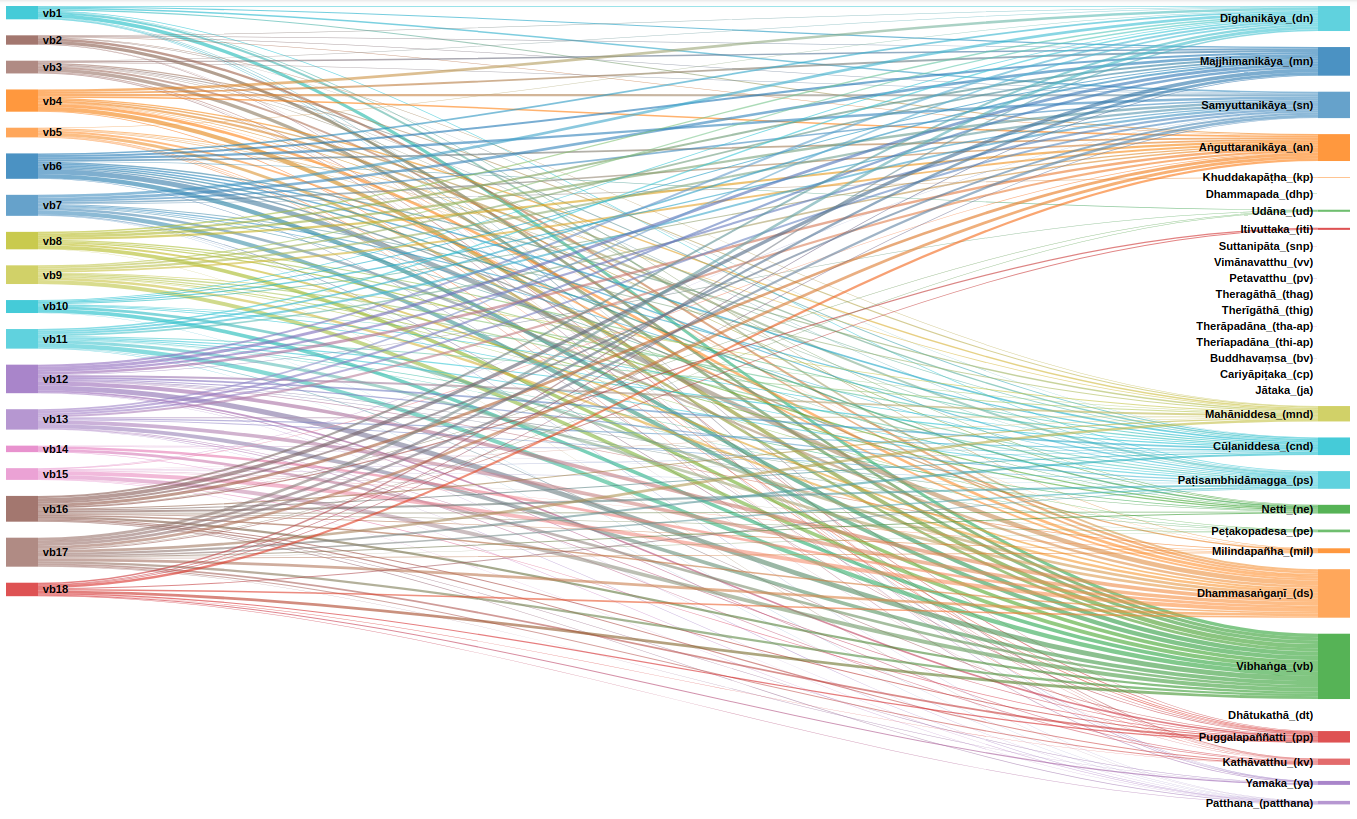
\includegraphics[width=\linewidth]{vbmatches.png}
\captionof{figure}{Sankey chart of all matches between the Vibhaṅga and other texts}
\label{vbmatches}

\subsubsection{Paṭṭhāna (patthana)}
Paṭṭhāna (Conditional Relations) sets out a simple mātikā listing 24 kinds of condition. For example, the first is the “root condition” (hetupaccayo), dealing with how acts are caused by the unwholesome roots of greed, hate, and delusion, or their opposites. This mātikā is then applied to the mātikās of Dhammasaṅgaṇī, creating a bewildering complexity of possible combinations. The Paṭṭhāna is always heavily abbreviated, but if it were to be fully spelled out, it would probably be the largest book ever created, with many billions of combinations. The Dhammasaṅgaṇī and the Paṭṭhāna bookend the Abhidhamma collection, the first dealing with phenomena, the latter with their relations. While method and the details have expanded considerably, the approach can be seen as a detailed application of the underlying principles of dependent origination.

The Paṭṭhāna has the largest AWL of all the Abhidhamma books. It is a work in itself and although it draws on the Dhammasaṅgaṇī, the main bulk of the text is unique in that it does not have many connections with other texts. Most notably, the text it has most matches with outside itself is the Parivāra.\\

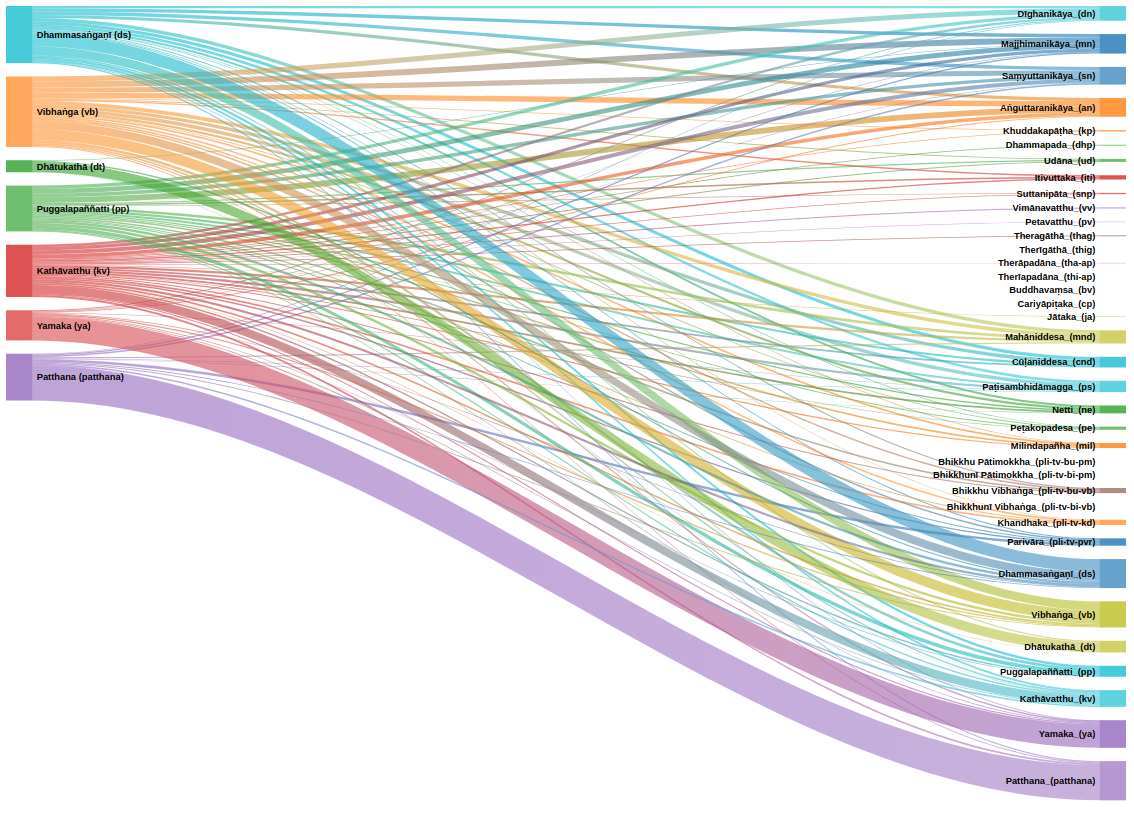
\includegraphics[width=\linewidth]{abhidhamma.png}
\captionof{figure}{Sankey chart of all matches between the Abhidhamma collections and other texts}
\label{abhidhamma}

\medskip
This figure also shows that all Abhidhamma collections are highly repetitive, given the high number of matches between the various chapters.

The Paṭṭhāna finds itself at the end of the Abhidhamma collection and with such a high AWL, I would consider it the latest book of the Abhidhamma, probably close to or overlapping with the development of the commentaries.

\subsubsection{Aṭṭhakathā (atk)}
The Aṭṭhakathā is a collection of Theravadin Buddhist commentaries to the canonical Theravadin Tipitaka. As noted before, the major commentaries were based on earlier ones, now lost, in Prakrit and Sinhala, which were written down at the same time as the Canon, in the last century BCE. Some material in the commentaries is found in canonical texts of other schools of Buddhism, suggesting an early common source. This can also explain why the AWL value of the Aṭṭhakathā on Suttas and Vinaya are relatively low and more in line with the other late texts like the Vinaya and Abhidhamma.

The contents of collected editions of the Theravadin commentaries, compiled from the fourth century CE onwards, varies between editions. 

